Однако кристаллы альдолазы так и не выпали.
Чтобы получить кристаллы, раствор довели до комнатной температуры,
после чего поставили в холодильник. Раствор помутнел.

Затем раствор центрифугировали (20 минут при 30000g).
Объем супернатанта составил 410 ml.
Из супернатанта отобрали 500 мкл для анализов (\emph{проба 3}).
Осадок перенесли в стеклянный стаканчик путем суспендирования осадка
в растворе сульфата аммония со степенью насыщения 0.5,
приготовленного на 25 mM глицил-глициновом буфере, рН=7.5.
Затем осадок, содержащий альдолазу, поместили в холодильник (\emph{проба 4}).
Объем осадка составил примерно 8 ml.

\section{Определение концентрации белка}

\subsection{Спектрофотометрическое опредление концентраций}
$$ A_{280} = \epsilon c l $$
Проверяли, что $ 0.1 < A_{280} < 1 $.

Для всех проб действовали по следующей схеме:
\begin{enumerate}
\item набирали 2 ml бидистилированной воды в кювету
\item обнуляли прибор
\item доливали 50 µl раствора из пробы
    (данное количество было подобрано, чтобы разведение составило 41).
\item снимали значение $A_{280}$
\end{enumerate}
Таким образом, разведение равно 41.
Было допущено, что удельное поглощение $\epsilon = 1$ для белка.
Для пробы 4 было использовано литературное значение $\epsilon = 0.91$.
Толщина кюветы $l = 1 \text{cm}$.
Таким образом, концентрация белка в пробе равна: $ c=41 \cdot A $ [mg/ml].

\begin{table}[htbp]
\caption{Концентрация белка, определенная спектрофотометрическим способом}
\begin{tabular}{|c|c|c|}
\hline
Проба & A & C[mg/ml] \\
\hline
\multirow{2}{*}{1} & 0.49 & 20 \\
& 0.54 & 22 \\
\hline
\multirow{2}{*}{2} & 0.177 & 7.257 \\
& 0.2 & 8.2 \\
\hline
3 & 0.154 & 6 \\
\hline
4 & 0.148 & 32.7 \\
\hline
\end{tabular}
\label{table-spm}
\end{table}

\subsection{Введение в метод Брэдфорд}
Метод Брэдфорд -- один из колориметрических методов количественного определения белков в растворе
(особенно с низкой концентрацией).
Данный метод основан на связывании белками красителя Coomassie Brilliant Blue G-250 \cite{bradford-1}.
Механизм связывания Coomassie заключается во взаимодействии анионной формы красителя с белком \cite{bradford-2}.

\begin{figure}[htbp]
\def\svgwidth{0.7\linewidth}\input{img/Coomassie_Brilliant_Blue_G-250.pdf_tex}
\caption{Краситель Coomassie Brilliant Blue G-250}
\end{figure}

Связывание с белком осуществляется за счет электростатического взаимодействия сульфонильных групп
красителя с аминокислотными остатками белка.
Связывание красителя Coomassie происходит преимущественно с аргининовым остатком и в меньшей степени с
остатками гистидина, лизина, тирозина, триптофана и фенилаланина.
Количество связей, образуемых между Coomassie и белком, зависит от количества положительно заряженных групп,
расположенных в молекуле белка.
Считается, что 1.5-3 молекулы красителя связываются одной положительно заряженной группой \cite{bradford-3}.
Исходный кислый раствор Coomassie имеет максимум поглощения при длине волны 465 нм.
После связывания с белком и изменения окраски максимум поглощения смещается к 595 нм
(рисунок~\ref{fig-shift}).

\begin{figure}[htbp]
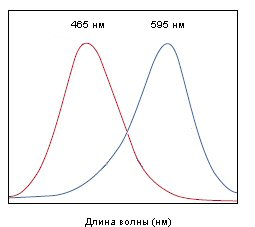
\includegraphics[width=0.4\linewidth]{bradford-shift}
\caption{Сдвиг максимума поглощения после связывания Coomasie с белком}
\label{fig-shift}
\end{figure}

\subsection{Калибровка для метода Брэдфорд}
\label{A0k}

Состав пробы: 1.9 ml Брэдфорд, буфер и БСА с концентрацией 0.4 mg/ml.

Под экспериментальные данные была подогнана линейная зависимость
(рисунок~\ref{fig-calibration}).

\begin{figure}[htbp]
\input{gnuplot/bsa}
\caption{Калибровка для метода Брэдфорд.
    На графике показана зависимость $A_{595}$ от содержания белка в кювете}
\label{fig-calibration}
\end{figure}

\subsection{Определение концентраций белка методом Брэдфорд}

Учитывая примерные концентрации, полученные спектрофотометрическим методом,
раствор из проб развели так, чтобы количество белка лежало в пределах
калибровочной кривой (0.1 -- 0.2).

Концентрация белка в пробе (mg/ml):

$$ c = \frac{m \cdot N}{V_c} $$
где $m$ -- содержание белка в кювете (µg),
$N$ -- разведение,
$V_c$ -- объем кюветы (2 ml).

\begin{table}[htbp]
\caption{Концентрация белка, определенная способом Брэдфорд}
\begin{tabular}{|c|c|}
\hline
Проба & C[mg/ml] \\
\hline
1 & 15.6 \\
\hline
\multirow{2}{*}{2} & 17.6 \\
& 25.1 \\
\hline
3 & 6.2 \\
\hline
\end{tabular}
\label{table-bredford}
\end{table}

